%
% File: chap01.tex
% Author: Zeller Quentin
% Description: Introduction
%
%\let\textcircled=\pgftextcircled
\chapter{HBBTV}
\label{chap:HBBTV}

\initial{H}ybrid Broadcast Broadband TV, plus connu sous l'acronyme HbbTV est un standard permettant le partage d'information et de services en compl�ment a un flux multim�dias destin�s a l'utilisateur final. \\

Il fait partie des outils ou protocols TV OTT, acronyme signifiant t�l�vision Over The Top ou services par contournement en fran�ais et qui d�finissent les contenus ne passant pas par le bouquet propos� par l'op�rateur internet / t�l�vision. C'est donc l'antith�se de la t�l�vision lin�aire, mode de consommation traditionnel. \cite{OTT}\\
\begin{figure}
%	HbbTV - Broadcast \("redbutton"\) vs broadband \("Web TV\).
	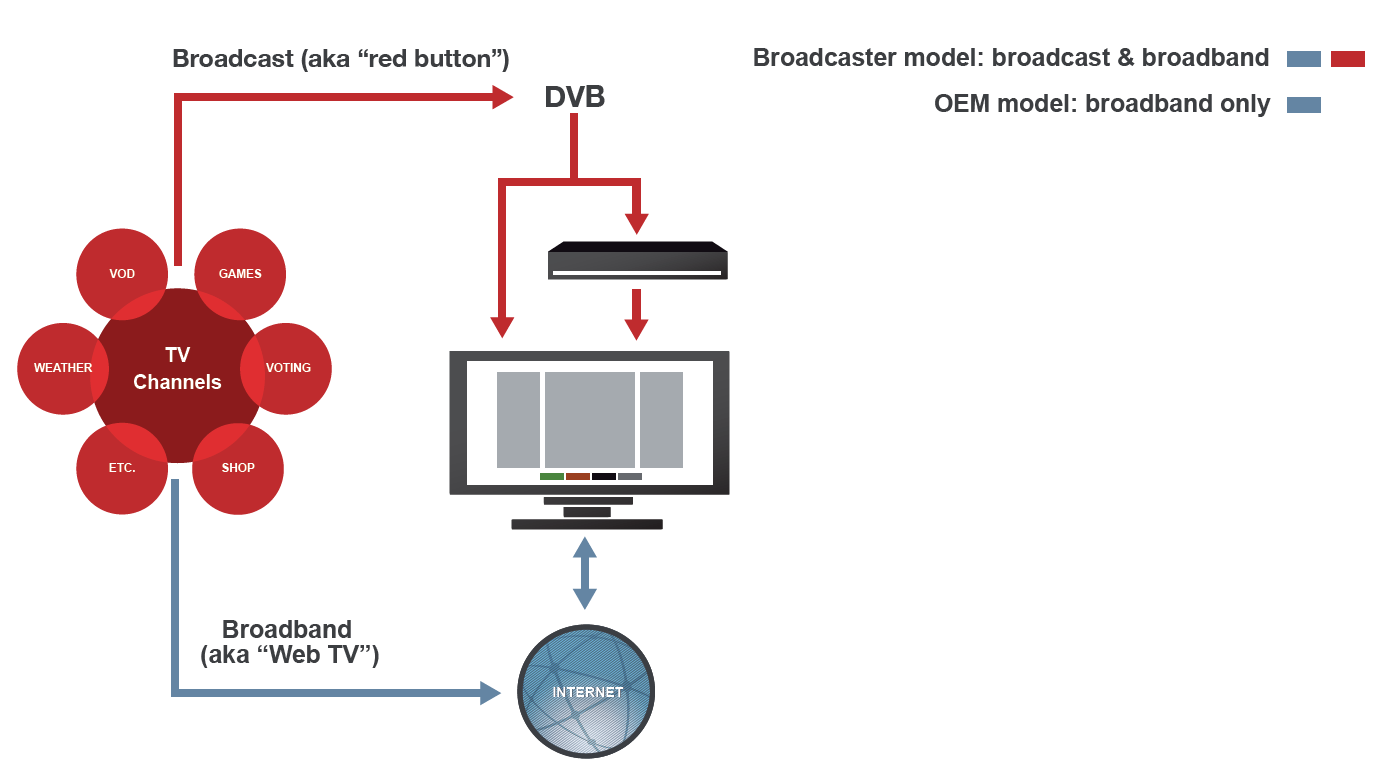
\includegraphics[width=\linewidth]{fig01/hbbtv-red-web}
	\caption{HbbTV Broadband vs Broadcast}
	\label{fig:hbbtv1}
\end{figure}

%=======
\section{Fonctionnement g�n�ral}
\label{sec:sec01}
\section{Environnement de d�veloppement}
\label{sec:sec02}

Begins a section.

\subsection{Emulateurs}
\label{subsec:subsec02}

Begins a subsection.

%A figures matrix.
\begin{figure}[t!]
\centering
\begin{minipage}{3.3cm}
    \centering
    \subtop[]{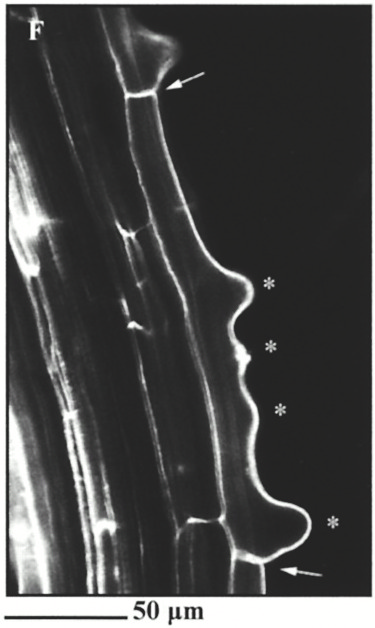
\includegraphics[height=0.28\textheight]{fig01/Nswellings}\label{sf:multiRH02a}}
\end{minipage}
\hspace{0.5cm}
\begin{minipage}{3.3cm}
    \centering
    \subtop[]{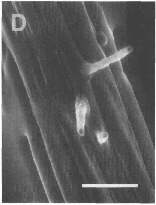
\includegraphics[height=0.27\textheight]{fig01/Mswellings}\label{sf:multiRH02b}}
\end{minipage}
\hspace{1.3cm}
\begin{minipage}{3.3cm}
    \centering
    \subtop[]{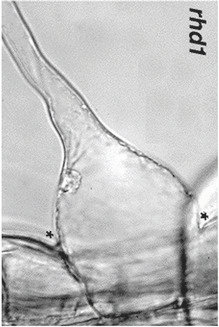
\includegraphics[height=0.27\textheight]{fig01/rhd1}\label{sf:multiRH02c}}
\end{minipage}
\\ \vspace{0.1cm}
\begin{minipage}{10cm}
    \centering
    \subtop[]{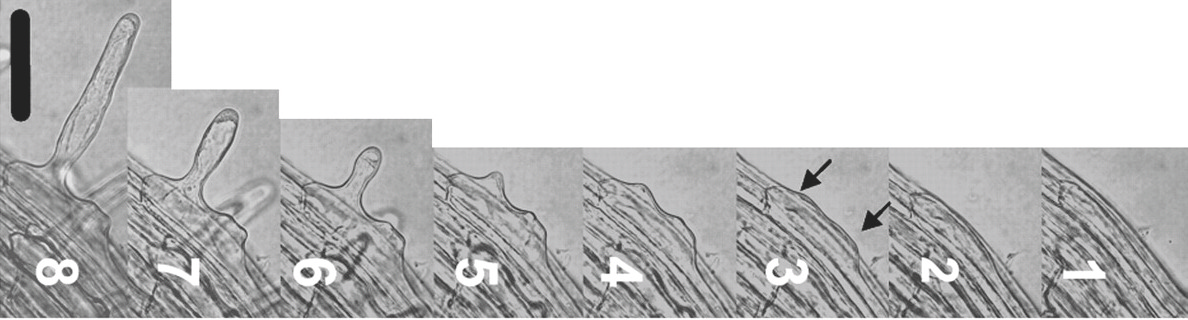
\includegraphics[height=0.145\textheight]{fig01/mutantrhd6}\label{sf:multiRH02d}}
\end{minipage}
\\ \vspace{0.1cm}
\begin{minipage}{10cm}
    \centering
    \subtop[]{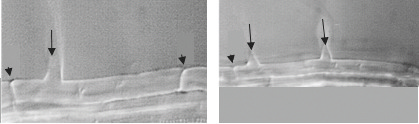
\includegraphics[height=0.16\textheight]{fig01/auxab}\label{sf:multiRH02e}}
\end{minipage}
\mycaption[Hair-forming mutant cells.]{(a) A mutant RH cell. Asterisks show multiple sites of RH initiation in a single root hair cell (indicated by the arrows). Figure reproduced from \cite{rigas01}. (b)~Hair-forming cell with three RH initiation locations. The bar represents $50\mu m$. Figure reproduced from \cite{massuci01}. (c) Large bump in mutant {\itshape rhd1}. Figure reproduced from \cite{griersonRH}. (d) Mutant overexpressing gene {\itshape ROP2}; from right-hand to left-hand, numbers indicate progressive snapshots at different times. RH initiation sites are indicated by the arrows. The bar represents $75\mu m$. Figure reproduced from~\cite{mjones01}. (e)~Mutants affected by auxin. On the left-hand side, RH site is farther away from the apical end (left arrow cap); on the right-hand side, multiple RH locations (arrows). Figure reproduced from~\cite{payne01}.}
\label{fig:multiRH02}
\end{figure}

% A single figure
\begin{figure}[t!]
	\centering
	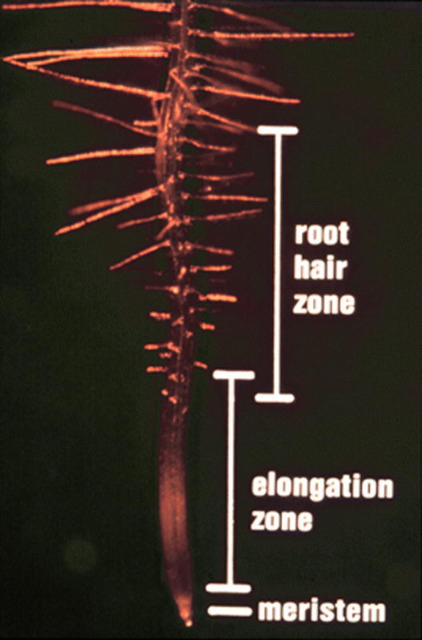
\includegraphics[height=0.35\textheight]{fig01/devepzones}
	\mycaption[Developmental zones of an Arabidopsis root.]{Developmental zones of an Arabidopsis root. Figure reproduced from \cite{griersonRH}.}
	\label{fig:RHP02}
\end{figure}

%=========================================================